\documentclass[11pt]{article}
\usepackage{graphicx}
\usepackage{amsmath,systeme}
\graphicspath{ {./obrazky/} }
\begin{document}
	
	\begin{titlepage}
		\begin{center}	
			\Huge{Vysoké učení technické v Brně}
			\huge{Fakulta informačních technologií}
			
\includegraphics[width=\linewidth]{fit.png}
			\vspace{1cm}
			\huge{Elektronika pro informační technologie}
			\vspace{1cm}
			\huge{2018/2019}\\
			\vspace{2cm}
			\huge{\textbf{Semestrální projekt}}\\
			\vspace{5cm}
	    	\Large{Matěj Drábek (xdrabe08)~~~~~~~~~~~~~~~~~~ Brno 19.12 2018}
		\end{center}	
	\end{titlepage}

\section*{1.C}
\large{Zadání:}\\
$U_1 = 100V$
$U_2 = 80V$\\
$R_1 = 450\Omega$
$R_2 = 810\Omega$
$R_3 = 190\Omega$
$R_4 = 220\Omega$
$R_5 = 220\Omega$
$R_6 = 720\Omega$
$R_7 = 260\Omega$
$R_8 = 180\Omega$\\
$U_{r3} = ?$
$I_{r3} = ?$\\
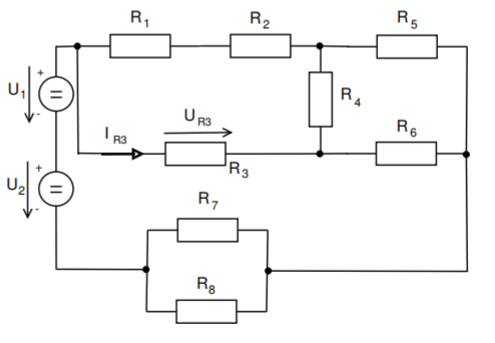
\includegraphics[width=0.8\linewidth]{priklad1_zadani.png}\\
\centerline {\huge{Řešení metodou postupného zjedodušování}}\\
Označení uzlů pro transfiguraci (trojuhelník $\Rightarrow$ hvězda):\\
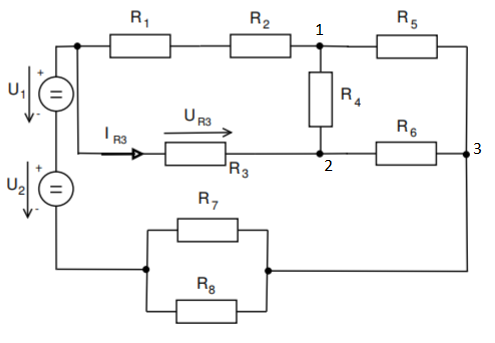
\includegraphics[width=0.8\linewidth]{priklad1_oznaceniBodu.png}\\
Provedení transfigurace a spojení $R_1$ a $R_2$:\\
$$R_{12} = R_1 + R_2 = 450 + 810 = 1260$$
$$R_A = \frac{R_4 * R_5}{R_4 + R_6 + R_5} = \frac{220*220}{220+220+720} = 41.7241\Omega$$
$$R_B = \frac{R_4 * R_6}{R_4 + R_6 + R_5} = \frac{220*720}{220+220+720} = 136.5517\Omega$$
$$R_C = \frac{R_6 * R_5}{R_4 + R_6 + R_5} = \frac{220*720}{220+220+720} = 136.5517\Omega$$
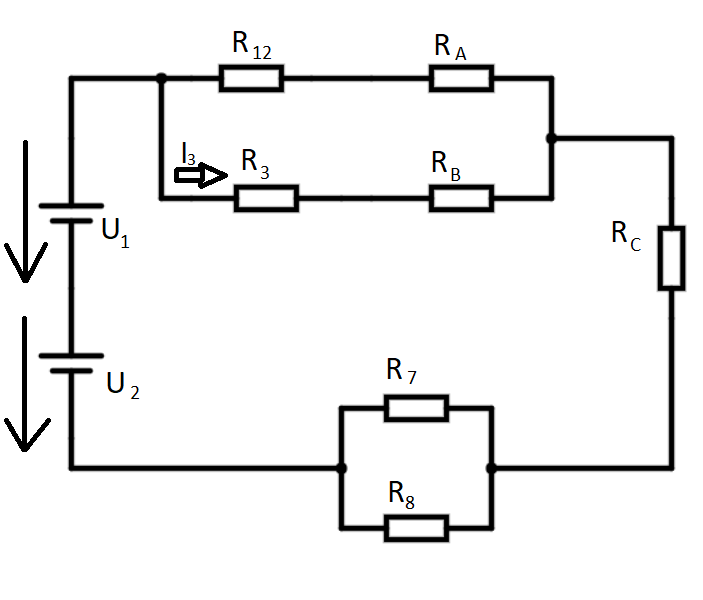
\includegraphics[width=0.8\linewidth]{priklad1_transfigurace.png}\\
\newpage
Sériové spojení $R_{12}$ s $R_A$ a $R_3$ s $R_B$ a Paralelní spojení $R_7$ s $R_8$
$$R_{12A} = R_{12} + R_A = 1260 + 41.7241 = 1300.7241\Omega$$
$$R_{3B} = R_3 + R_A = 190 + 136.5517 = 326.5517\Omega$$
$$R_{78} = \frac{R_7 * R_8}{R_7 + R_8} = \frac{260 * 180}{260 + 180} = 106.3636\Omega$$
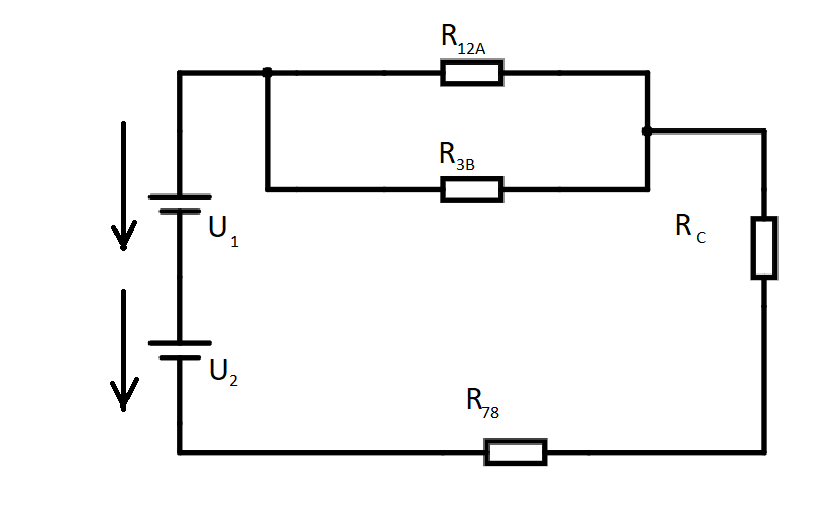
\includegraphics[width=0.8\linewidth]{priklad1_zjednoduseni1.png}\\
Sériové spojení $R_{78}$ s $R_C$, Paralelní spojení $R_12A$ s $R_3B$ a spojení zdrojů napětí
$$R_{78C} = R_{78} + R_{C} = 106.3636 + 136.5517 = 242.9153$$
$$R_{123AB} = \frac{R_{12A} * R_{3B}}{R_{12A} + R_{3B}} = \frac{1300.7241 * 326.5517}{1300.7241 + 326.5517} = 261.0184\Omega$$
$$U_{12} = U_1 + U_2 = 100 + 800 = 180V$$
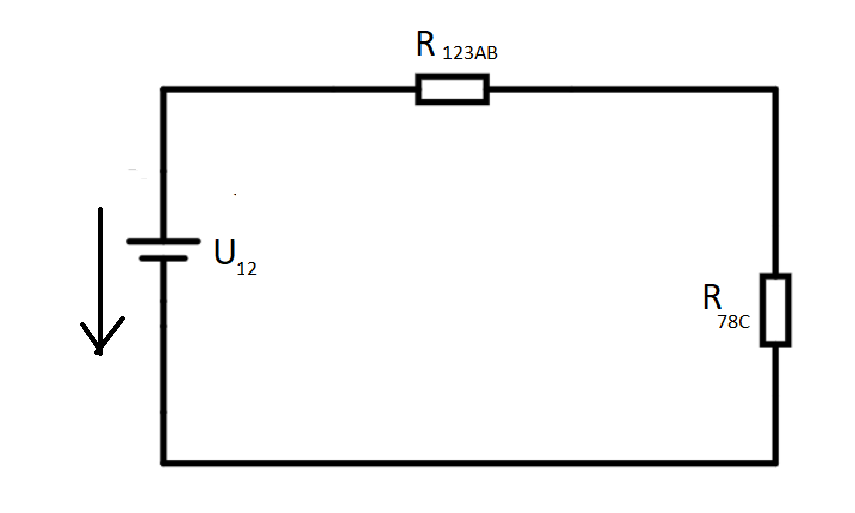
\includegraphics[width=0.8\linewidth]{priklad1_zjednoduseni2.png}\\
Sériové spojení $R_{123AB}$ s $R_{78C}$
$$R_{EKV} = R_{123AB} + R_{78C} = 261.0184 + 242.9153 = 503.9337$$
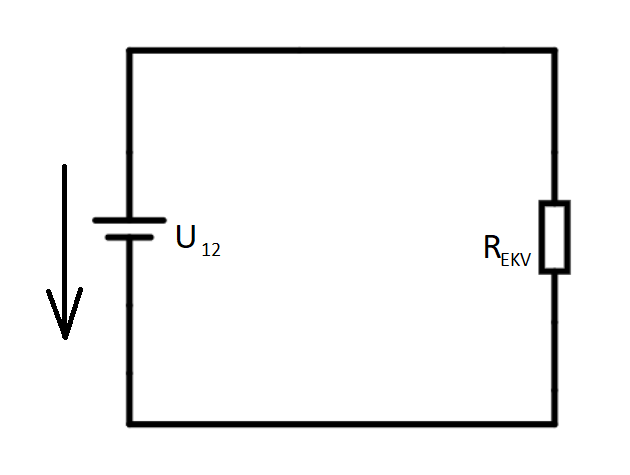
\includegraphics[width=0.8\linewidth]{priklad1_zjednoduseni3.png}\\
Celkový proud $I$:
$$I = \frac{U}{R_{EKV}} = \frac{180}{503.9337} = 0.3571A$$
Nyní můžeme zpětně dopočítat napětí a proud na rezistoru $R_3$
$$U_{123AB} = I * R_{123AB} = 0.3571 * 261.0184 = 93.2096$$
$$I_3 \equiv I_{3B} = \frac{U_{123AB}}{R_{3   B}} = \frac{93.2096}{326.5551} = 0.2854$$
$$U_3 = I * R_3 = 0.2854 * 190 = 54.226$$
\newpage
\section*{2.B}
Zadání:\\
$U = 100V$\\
$R_1 = 50\Omega$
$R_2 = 310\Omega$
$R_3 = 610\Omega$
$R_4 = 220\Omega$
$R_5 = 570\Omega$\\
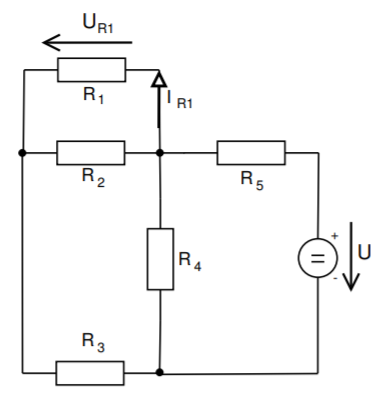
\includegraphics[width=0.7\linewidth]{priklad2_zadani.png}\\
\centerline{\huge{Řešení pomocí Théveninovy věty}}
\newpage
Výpočet $R_i$:\\
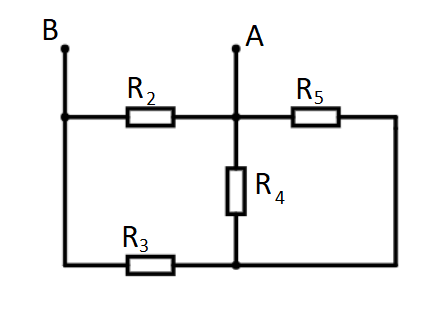
\includegraphics[width=0.7\linewidth]{priklad2_Ri.png}
$$R_i = \frac{(\frac{R_5 * R_4}{R_5 + R_4} + R_3) * R_2}{(\frac{R_5 * R_4}{R_5 + R_4} + R_3) + R_2} = \frac{(\frac{570 * 220}{570 + 220} + 610) * 310}{(\frac{570 * 220}{570 + 220} + 610) + 310} = 220.9141$$
Výpočet $U_i$:\\
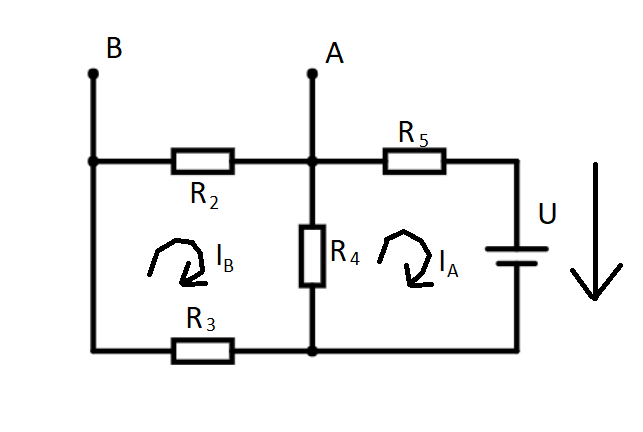
\includegraphics[width=0.7\linewidth]{priklad2_Ui.png}\\
Vypočítáme $I_B$ metodou smyčkových proudů:\\
\begin{equation*}
  \systeme{
  U + R_4*I_A - R_4 * I_B + R_5 * I_A  = 0,
  R_2 * I_B + R_3 * I_B + R_4 * I_B - R_4 * I_B = 0
  }
\end{equation*}
\begin{equation*}
  \systeme{
  100 + 220I_A - 220I_B + 570I_A  = 0,
  310I_B + 610I_B + 220I_B - 220I_B = 0
  }
\end{equation*}
\begin{equation*}
  \systeme{
  790I_A - 220I_B  = -100,
  - -220I_A + 1140I_B = 0 / * 3.590909091
  }
\end{equation*}
\begin{equation*}
  \systeme{
  790I_A - 220I_B  = -100,
  - -790I_A + 4093.6363I_B = 0
  }
\end{equation*}
$$3873.6363I_B = - 100$$
$$I_B = 0.02581A$$
$$U_i = U_2 = R_2 * I_B = 310 * 0.02581 = 8.00281V $$
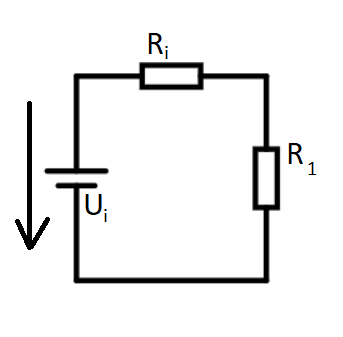
\includegraphics[width=0.7\linewidth]{priklad2_nahrazeni.png}\\
$$I_i = \frac{U_i}{R_i + R_1} = \frac{8.00281}{220.9141 + 50} = 0.02964A$$
$$U_1 = R_1 * I_i = 1.48200V$$
$$I_1 = \frac{U_1}{R_1} = \frac{1.48200}{50} = 0.02964A$$
\end{document}
